\chapter{Results}
\label{ch:results}

All numbers are means over the runs named in each caption. $p$-values come from the paired Wilcoxon signed-rank test of Section~\ref{sec:tests}. Tables marked as generated are produced by \texttt{thesis/scripts/make\_figures.py} directly from the stored run records.

\section{Experiments Run}
\begin{table}[H]
\centering
\caption{Inventory of experiments.}
\label{tab:run-status}
\small
\begin{tabularx}{\textwidth}{@{}>{\raggedright\arraybackslash}p{3.1cm} Y r >{\raggedright\arraybackslash}p{2.6cm}@{}}
\toprule
\textbf{Experiment} & \textbf{Setup} & \textbf{Runs} & \textbf{Purpose} \\
\midrule
Baseline (v1) & Llama 8B (5 scenarios), Qwen 7B (2) & 63 & RQ1 \\
v2 & Output limit 4096 tokens & 63 & Truncation check \\
v3 & Stage definitions in prompt & 63 & Stage vocabulary \\
v4 & Per-process triage added & 63 & False-positive control \\
v5 & GoT with cross-segment links & 21 & Aggregate mechanism \\
Scale (v4 setup) & Qwen 32B, Llama 70B (AWQ) & 63 & Model size \\
Scale, no triage & Llama 70B & 63 & Input-length effect \\
Primus (v4 setup) & Llama-Primus-Reasoning 8B & 45 & RQ3 \\
\bottomrule
\end{tabularx}
\end{table}

\section{Baseline: Topology Comparison (RQ1)}
Table~\ref{tab:baseline} and Figure~\ref{fig:baseline} give the baseline over all 63 runs (21 per method).

\begin{table}[H]
\centering
\caption{Baseline results by method (mean of 21 runs each).}
\label{tab:baseline}
\small
\begin{tabularx}{\textwidth}{@{}l C C C C C C@{}}
\toprule
\textbf{Method} & \textbf{Precision} & \textbf{Recall} & \textbf{Event F$_1$} & \textbf{Stage recall} & \textbf{Partial SR} & \textbf{Halluc.} \\
\midrule
CoT & 0.179 & 0.200 & 0.181 & 0.049 & 0.096 & 0.095 \\
ToT & 0.235 & 0.263 & 0.234 & 0.018 & 0.115 & 0.190 \\
GoT & 0.223 & 0.375 & 0.267 & 0.061 & 0.192 & 0.157 \\
\bottomrule
\end{tabularx}
\end{table}

\begin{figure}[H]
\centering
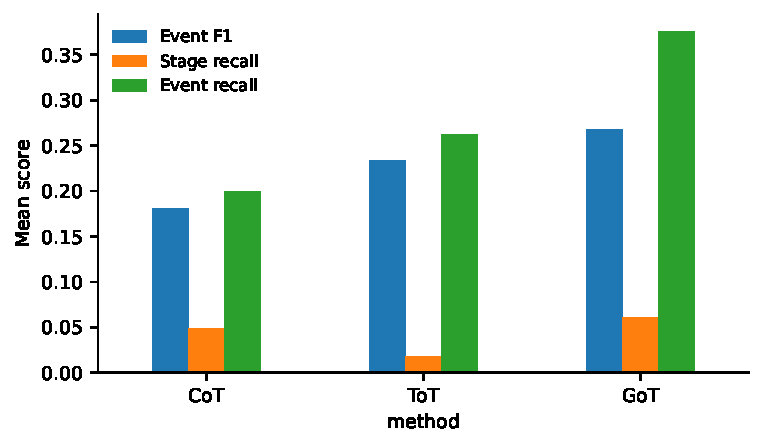
\includegraphics[width=0.62\textwidth]{fig_baseline_methods}
\caption{Baseline mean event F$_1$, stage recall and event recall by method.}
\label{fig:baseline}
\end{figure}

GoT has the highest mean event recall and F$_1$, and ToT the highest precision. For stage recall no pairwise difference is significant, while GoT's event-recall advantage is significant before multiple-test correction (Section~\ref{sec:res-tests}). Table~\ref{tab:bymodel} splits the same runs by model; Qwen 2.5 7B has an exact stage recall of exactly 0.000 under CoT and ToT.

\begin{table}[H]
\centering
\caption{Baseline results by model and method.}
\label{tab:bymodel}
\small
\begin{tabularx}{\textwidth}{@{}l l C C C C@{}}
\toprule
\textbf{Model} & \textbf{Method} & \textbf{Precision} & \textbf{Recall} & \textbf{Event F$_1$} & \textbf{Stage recall} \\
\midrule
Llama 3.1 8B & CoT & 0.152 & 0.177 & 0.154 & 0.069 \\
 & ToT & 0.217 & 0.258 & 0.218 & 0.025 \\
 & GoT & 0.188 & 0.324 & 0.222 & 0.053 \\
\addlinespace
Qwen 2.5 7B & CoT & 0.245 & 0.256 & 0.246 & 0.000 \\
 & ToT & 0.280 & 0.274 & 0.274 & 0.000 \\
 & GoT & 0.312 & 0.505 & 0.380 & 0.079 \\
\bottomrule
\end{tabularx}
\end{table}

By scenario (Figure~\ref{fig:heatmap}), mean event F$_1$ over all baseline runs is 0.362 for WS12, 0.280 for Ubuntu, 0.116 for Sidewinder, 0.107 for FIN6 and 0.084 for APT29. The three scenarios that share one Windows~10 log score far lower than the two that do not.

\begin{figure}[H]
\centering
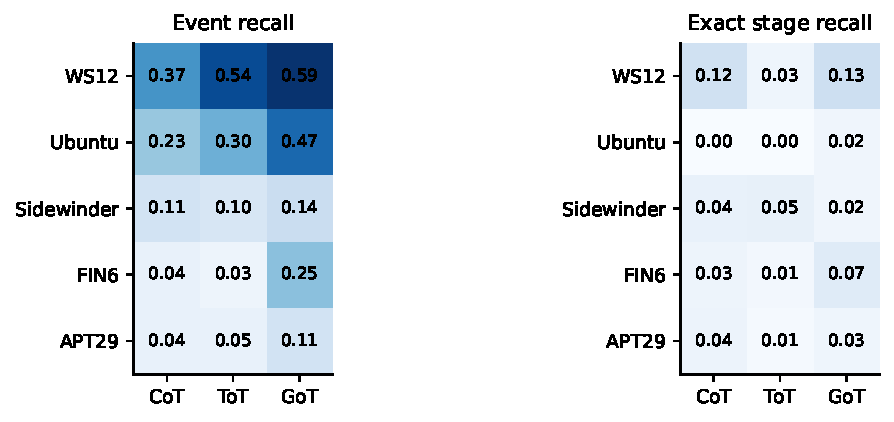
\includegraphics[width=0.85\textwidth]{fig_scenario_heatmap}
\caption{Baseline event recall and exact stage recall by scenario and method.}
\label{fig:heatmap}
\end{figure}

\section{Tests of the Hypothesis}
\label{sec:res-tests}
Table~\ref{tab:tests} applies the paired test of Section~\ref{sec:tests} to every experiment. $\Delta$ is the mean difference (first method minus second) over the $n$ matched cells.

\begin{table}[H]
\centering
\caption{Paired Wilcoxon tests between topologies (generated). $\Delta$ is the mean difference; $n$ is the number of matched (scenario, model, seed) cells.}
\label{tab:tests}
\footnotesize
\resizebox{\textwidth}{!}{\begin{tabular}{@{}llrrrrrrr@{}}
\toprule
 & & \multicolumn{2}{c}{GoT vs CoT} & \multicolumn{2}{c}{GoT vs ToT} & \multicolumn{2}{c}{ToT vs CoT} & \\
\cmidrule(lr){3-4}\cmidrule(lr){5-6}\cmidrule(lr){7-8}
Experiment & Metric & $\Delta$ & $p$ & $\Delta$ & $p$ & $\Delta$ & $p$ & $n$ \\
\midrule
Baseline (v1) & Stage recall & +0.011 & 0.386 & +0.043 & 0.113 & -0.031 & 0.161 & 21 \\
 & Event recall & +0.175 & 0.009 & +0.113 & 0.023 & +0.063 & 0.278 & 21 \\
\addlinespace
v3 stage definitions & Stage recall & +0.089 & 0.049 & +0.071 & 0.256 & +0.017 & 0.445 & 21 \\
 & Event recall & +0.166 & 0.013 & +0.077 & 0.232 & +0.090 & 0.031 & 21 \\
\addlinespace
v4 triage & Stage recall & +0.022 & 0.727 & +0.042 & 0.102 & -0.020 & 0.328 & 21 \\
 & Event recall & +0.048 & 0.478 & +0.069 & 0.191 & -0.022 & 0.629 & 21 \\
\addlinespace
Scale: Qwen 32B, Llama 70B & Stage recall & +0.049 & 0.201 & +0.085 & 0.028 & -0.036 & 0.260 & 21 \\
 & Event recall & +0.142 & 0.007 & +0.149 & 0.006 & -0.007 & 0.975 & 21 \\
\addlinespace
Llama-Primus 8B & Stage recall & +0.030 & 0.348 & +0.019 & 0.600 & +0.011 & 0.684 & 15 \\
 & Event recall & +0.072 & 0.126 & -0.003 & 0.859 & +0.075 & 0.123 & 15 \\
\bottomrule
\end{tabular}
}
\end{table}

Of the 30 comparisons in the table, 8 have an uncorrected $p<0.05$, and they are not spread evenly across the two metrics.
\begin{itemize}
\item \textbf{Stage recall, the metric named in the hypothesis.} Only two of the 15 comparisons are below 0.05: GoT against CoT in v3 ($\Delta=+0.089$, $p=0.049$) and GoT against ToT in the scale experiment ($\Delta=+0.085$, $p=0.028$). In the baseline, v4 and Primus experiments GoT's advantage in stage recall is small and not significant ($p$ from 0.10 to 0.73).
\item \textbf{Event recall.} GoT is significantly higher than CoT in the baseline ($\Delta=+0.176$, $p=0.009$), v3 ($+0.167$, $p=0.013$) and scale ($+0.142$, $p=0.007$) experiments, and higher than ToT in the baseline ($+0.113$, $p=0.023$) and scale ($+0.149$, $p=0.006$) experiments. It is not significant under v4 or for Primus.
\end{itemize}
These are 30 tests, so some small $p$-values are expected by chance. After Bonferroni correction (threshold $0.05/30=0.0017$) none survives, and the smallest Holm-adjusted $p$ is 0.18. We also pair each seed of a scenario as a separate observation, which treats repeated runs on the same scenario as independent and makes the tests somewhat anti-conservative. The honest reading is therefore: the primary prediction (higher stage recall for GoT) is not confirmed, and H0 is not rejected; GoT does show a consistent \emph{direction} of higher event recall, which is not established as a real effect at this sample size.

\section{Comparison across Models and Topologies}
Figure~\ref{fig:modeltop} and Table~\ref{tab:modeltop} compare the five models under the same v4 setup for each topology. Qwen 7B and Llama 8B cover the cells described in Chapter~\ref{ch:protocol}; Qwen 32B and Llama 70B and Primus use the cells their context allows.

\begin{figure}[H]
\centering
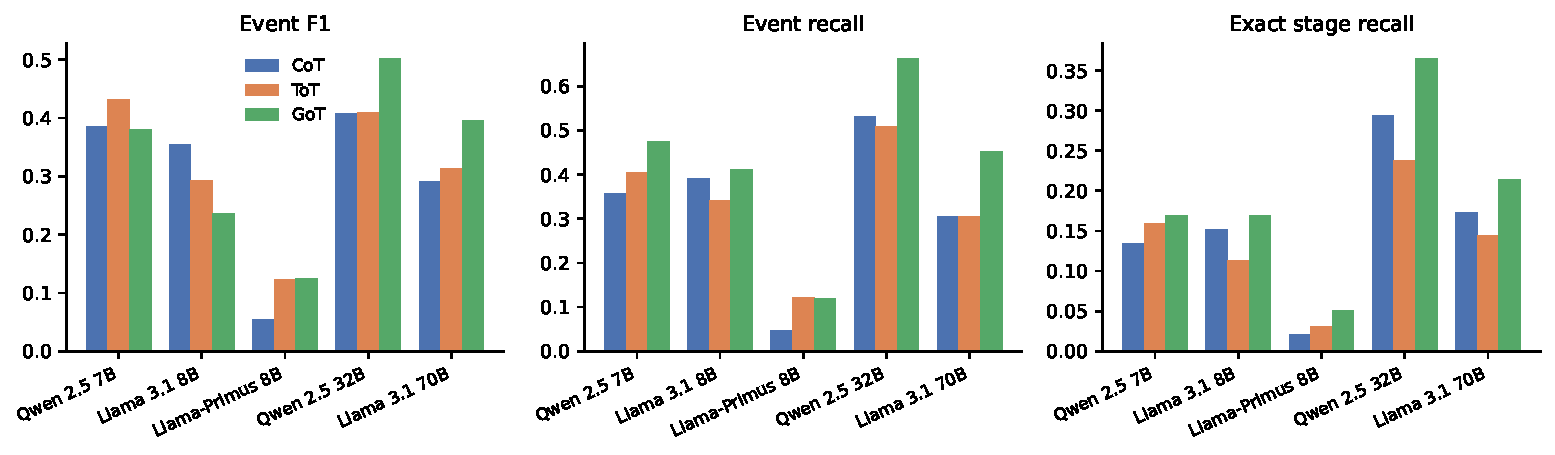
\includegraphics[width=\textwidth]{fig_model_topology}
\caption{Event F$_1$, event recall and exact stage recall for each model and topology under the v4 setup.}
\label{fig:modeltop}
\end{figure}

\begin{table}[H]
\centering
\caption{Models and topologies under the v4 setup (generated).}
\label{tab:modeltop}
\small
\begin{tabular}{@{}llrrrrr@{}}
\toprule
Model & Method & Runs & Precision & Recall & Event F$_1$ & Stage recall \\
\midrule
Qwen 2.5 7B & CoT & 6 & 0.493 & 0.357 & 0.385 & 0.135 \\
 & ToT & 6 & 0.538 & 0.405 & 0.432 & 0.159 \\
 & GoT & 6 & 0.340 & 0.475 & 0.380 & 0.169 \\
\addlinespace
Llama 3.1 8B & CoT & 15 & 0.343 & 0.390 & 0.355 & 0.151 \\
 & ToT & 15 & 0.289 & 0.341 & 0.294 & 0.114 \\
 & GoT & 15 & 0.203 & 0.410 & 0.236 & 0.169 \\
\addlinespace
Llama-Primus 8B & CoT & 15 & 0.097 & 0.048 & 0.055 & 0.021 \\
 & ToT & 15 & 0.134 & 0.123 & 0.124 & 0.031 \\
 & GoT & 15 & 0.190 & 0.119 & 0.124 & 0.050 \\
\addlinespace
Qwen 2.5 32B & CoT & 6 & 0.356 & 0.532 & 0.408 & 0.294 \\
 & ToT & 6 & 0.368 & 0.508 & 0.410 & 0.238 \\
 & GoT & 6 & 0.412 & 0.663 & 0.502 & 0.365 \\
\addlinespace
Llama 3.1 70B & CoT & 15 & 0.373 & 0.305 & 0.291 & 0.173 \\
 & ToT & 15 & 0.396 & 0.305 & 0.314 & 0.145 \\
 & GoT & 15 & 0.370 & 0.452 & 0.396 & 0.214 \\
\bottomrule
\end{tabular}

\end{table}

Two patterns stand out. First, the gaps between models are larger than the gaps between topologies within a model. Second, GoT has the highest event F$_1$ and stage recall for both large models (Qwen 32B: 0.502 and 0.365; Llama 70B: 0.396 and 0.214). GoT gives the best event recall for both large models and for Llama 8B, but its precision is lower than CoT's for the 7B and 8B models, so it finds more events at the price of more false ones.

\section{Improvement Rounds}
\label{sec:res-rounds}
Figure~\ref{fig:variants} shows the pooled effect of each change and Table~\ref{tab:vartests} gives the paired tests between successive variants.

\begin{figure}[H]
\centering
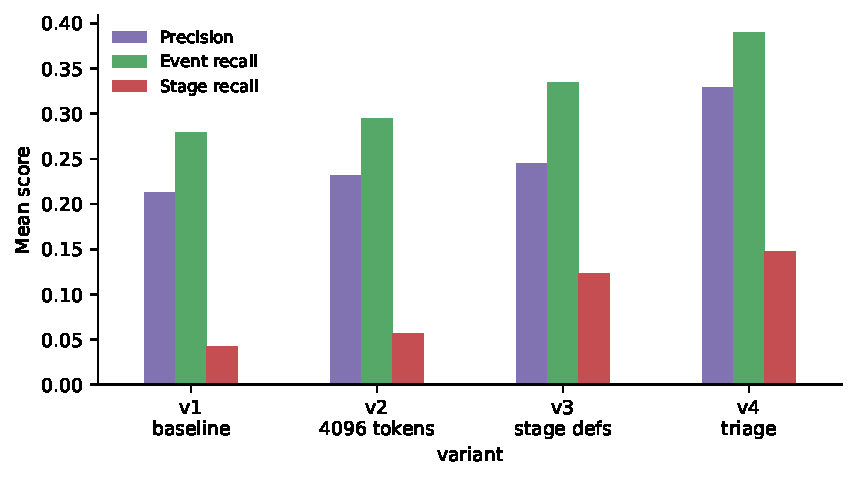
\includegraphics[width=0.72\textwidth]{fig_variants}
\caption{Pooled precision, event recall and stage recall by variant (63 runs each).}
\label{fig:variants}
\end{figure}

\begin{table}[H]
\centering
\caption{Paired tests between successive variants (generated).}
\label{tab:vartests}
\small
\begin{tabular}{@{}llrrrr@{}}
\toprule
Step & Metric & Before & After & $p$ & $n$ \\
\midrule
v1 to v2 & Stage recall & 0.043 & 0.056 & 0.1011 & 63 \\
 & Precision & 0.212 & 0.231 & 0.5467 & 63 \\
 & Event recall & 0.279 & 0.295 & 0.5439 & 63 \\
 & Event F1 & 0.227 & 0.239 & 0.6114 & 63 \\
v2 to v3 & Stage recall & 0.056 & 0.123 & 0.0015 & 63 \\
 & Precision & 0.231 & 0.245 & 0.4232 & 63 \\
 & Event recall & 0.295 & 0.334 & 0.0515 & 63 \\
 & Event F1 & 0.239 & 0.268 & 0.1038 & 63 \\
v3 to v4 & Stage recall & 0.123 & 0.147 & 0.3445 & 63 \\
 & Precision & 0.245 & 0.329 & 0.0400 & 63 \\
 & Event recall & 0.334 & 0.390 & 0.0762 & 63 \\
 & Event F1 & 0.268 & 0.325 & 0.0802 & 63 \\
\bottomrule
\end{tabular}

\end{table}

\begin{itemize}
\item \textbf{v2.} Raising the output limit changes nothing significantly, so truncation was not the bottleneck.
\item \textbf{v3.} Stage definitions double exact stage recall, from 0.056 to 0.123 ($p=0.0015$). This is the first significant result, and it addresses the labelling failure diagnosed in Chapter~\ref{ch:discussion}.
\item \textbf{v4.} Triage raises precision from 0.245 to 0.329 ($p=0.04$) and event F$_1$ from 0.268 to 0.325 ($p=0.08$). Detection barely moves (19.9\% to 21.3\% of true events found), so the gain comes mainly from fewer false positives.
\item \textbf{v5.} Giving GoT's Aggregate the cross-segment links raises GoT's event F$_1$ from 0.277 to 0.350 ($p=0.34$) and Llama's event recall from 0.41 to 0.54 ($p=0.055$). Neither is significant, and GoT still does not separate from CoT and ToT.
\end{itemize}

\section{Scaling the Model}
\label{sec:res-scale}
\begin{itemize}
\item Qwen 7B to 32B: exact stage recall 0.15 to 0.30 ($p=0.012$) and event recall 0.41 to 0.57 ($p=0.017$).
\item Llama 8B to 70B: precision 0.28 to 0.38 ($p=0.022$) and hallucination 0.19 to 0.06 ($p=0.001$), with recall flat. The 70B's stricter triage dropped 22\% of true attack events before reasoning began.
\item Llama 70B without triage is worse than with it: event F$_1$ falls from 0.33 to 0.23 ($p=0.0015$). Figure~\ref{fig:length} shows why: on the longest inputs the 70B's recall collapses.
\end{itemize}

\begin{figure}[H]
\centering
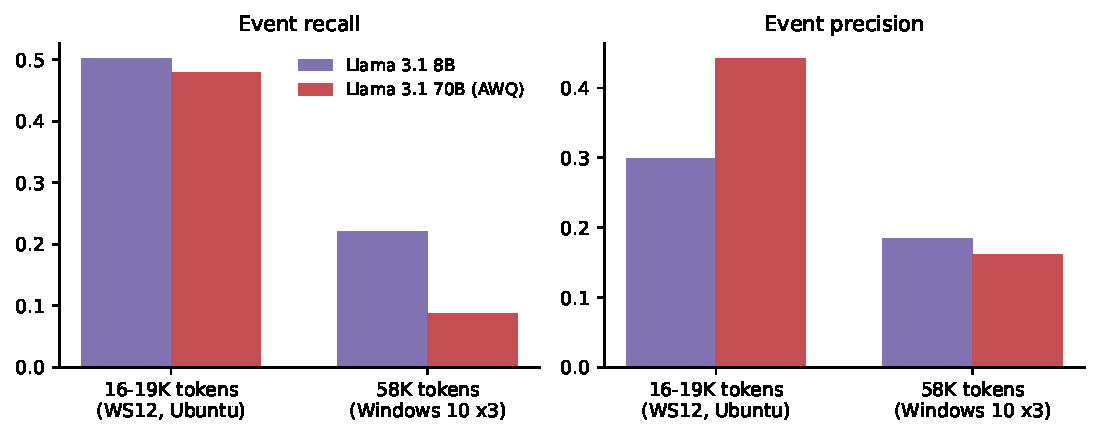
\includegraphics[width=0.85\textwidth]{fig_length_effect}
\caption{Llama 70B against Llama 8B without triage, split by input length. At 58K tokens the larger model's recall falls below the smaller one's.}
\label{fig:length}
\end{figure}

\section{Security-Tuned Model (RQ3)}
\label{sec:res-primus}
Llama-Primus-Reasoning has the size and architecture of Llama 3.1 8B but was further trained on cyber-security text and writes a reasoning trace before its answer. It was run under the v4 setup with the Llama 3.1 8B triage reused, so it and the comparison model read identical triaged evidence.

\begin{table}[H]
\centering
\caption{Llama-Primus-Reasoning by method, v4 setup (generated).}
\label{tab:primus}
\small
\begin{tabular}{@{}lrrrrr@{}}\toprule
Method & Precision & Recall & Event F$_1$ & Stage recall & Halluc.\\\midrule
CoT & 0.097 & 0.048 & 0.055 & 0.021 & 0.065\\
ToT & 0.134 & 0.123 & 0.124 & 0.031 & 0.031\\
GoT & 0.190 & 0.119 & 0.124 & 0.050 & 0.165\\
\midrule
All (45 runs) & 0.140 & 0.096 & 0.101 & 0.034 & 0.087\\
\bottomrule\end{tabular}

\end{table}

Over all 45 runs the security-tuned model is worse than Llama 3.1 8B on the same evidence (Table~\ref{tab:primusvs}). Paired over the 45 matched cells, event F$_1$ falls from 0.295 to 0.101, event recall from 0.381 to 0.096 and exact stage recall from 0.145 to 0.034; all are significant (recall and F$_1$ $p<0.001$, stage recall $p=0.0001$, precision $p=0.002$). Its hallucination rate is lower (0.087 against 0.194, $p=0.005$), but only because it reports fewer events.

\begin{table}[H]
\centering
\caption{Llama-Primus-Reasoning against Llama 3.1 8B, v4 setup, 45 matched runs each.}
\label{tab:primusvs}
\small
\begin{tabularx}{\textwidth}{@{}l C C C C C@{}}
\toprule
\textbf{Model} & \textbf{Precision} & \textbf{Recall} & \textbf{Event F$_1$} & \textbf{Stage recall} & \textbf{Halluc.} \\
\midrule
Llama 3.1 8B & 0.278 & 0.381 & 0.295 & 0.145 & 0.194 \\
Llama-Primus-Reasoning & 0.140 & 0.096 & 0.101 & 0.034 & 0.087 \\
\bottomrule
\end{tabularx}
\end{table}

\paragraph{Output-format failures.} 17 of the 45 runs (38\%) produced no parseable answer (Figure~\ref{fig:parse}): 10 of 15 CoT, 11 of 15 ToT and 7 of 15 GoT runs parsed. All Sidewinder runs scored zero. The model writes a long reasoning trace first (about 2,000 completion tokens for CoT and 10,000 for GoT), and because constrained decoding is off for it, nothing forces a valid answer. On the 28 runs that parsed, event F$_1$ is 0.126, event recall 0.120 and stage recall 0.031, so format failures explain part of the deficit but not all of it.

\begin{figure}[H]
\centering
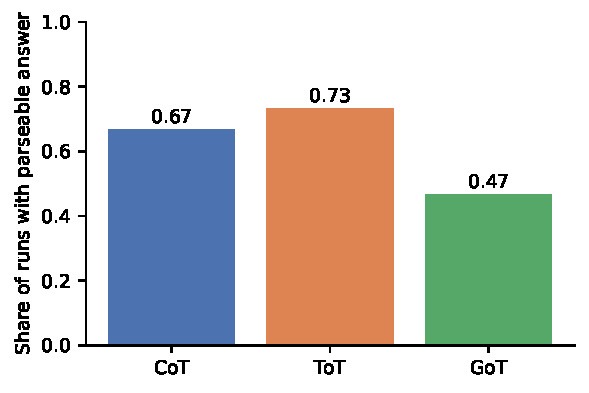
\includegraphics[width=0.5\textwidth]{fig_primus_parse}
\caption{Share of Llama-Primus-Reasoning runs that produced a parseable answer, by method (15 runs each).}
\label{fig:parse}
\end{figure}

\paragraph{Topology.} Within Primus, GoT and ToT have higher recall than CoT (0.119 and 0.123 against 0.048), but no comparison is significant (Table~\ref{tab:tests}).

\section{Accuracy and Cost}
\begin{figure}[H]
\centering
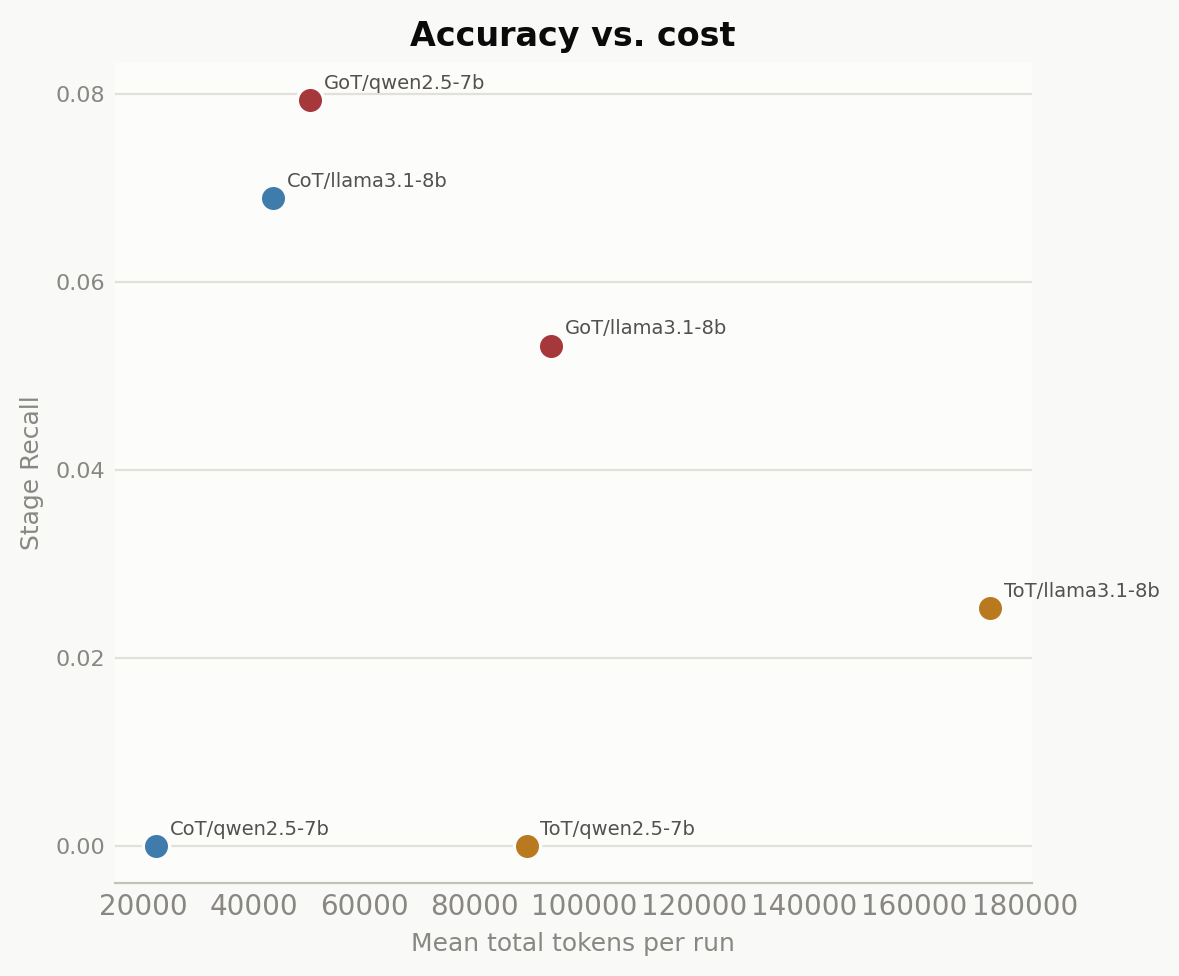
\includegraphics[width=0.78\textwidth]{fig_pareto}
\caption{Stage recall against cost for each method and model, from the baseline grid.}
\label{fig:pareto}
\end{figure}
Table~\ref{tab:cost} gives the baseline cost. GoT costs about twice the tokens of CoT and four times its wall-clock time, and ToT costs about four times the tokens of CoT. Neither extra cost buys a statistically significant accuracy gain in our data.

\section{Summary of Results}
\begin{enumerate}
\item On the primary metric, stage recall, GoT is not reliably better than CoT or ToT: 2 of 15 comparisons are below 0.05 uncorrected, and none survives correction.
\item GoT has consistently higher event recall (uncorrected $p<0.05$ in 5 of 10 comparisons against CoT and ToT), at the cost of lower precision at 7B--8B; none survives Bonferroni correction.
\item Stage definitions in the prompt (stage recall doubled), triage (precision $+0.08$) and model size (Qwen stage recall doubled) have larger and clearer effects than topology.
\item A security-tuned 8B model did worse than the general one, partly because of output-format failures.
\item Input length materially affects accuracy and is confounded with GoT's segmentation.
\end{enumerate}
